% Program Studi D-IV Komputasi Statistik
% Politeknik Statistika STIS

\documentclass[conference, a4paper]{IEEEtran_ID}
\IEEEoverridecommandlockouts
\usepackage{cite}
\usepackage{fancyhdr}
\usepackage{lastpage}
\usepackage{amsmath,amssymb,amsfonts}
\usepackage{algorithmic}
\usepackage{graphicx}
\usepackage{textcomp}
\usepackage{xcolor}
\def\BibTeX{{\rm B\kern-.05em{\sc i\kern-.025em b}\kern-.08em
    T\kern-.1667em\lower.7ex\hbox{E}\kern-.125emX}}

\pagestyle{fancy}
\fancyhf{}
\lhead{}
\rhead{\footnotesize{Villalobos, E. (2020)}}
\lfoot{}
\rfoot{\thepage { /} \pageref{LastPage}}
\renewcommand{\headrulewidth}{0pt}
\renewcommand{\footrulewidth}{0pt}


\begin{document}

% Elemen judul proposal
\title{\huge{La importancia visualización de datos \\ 
y algunas recomendaciones.} % Elemen subjudul proposal
}

% Elemen nama penulis
\author{
\IEEEauthorblockN{\Large{Elena Villalobos Nolasco}}\vspace{0.6em}
\IEEEauthorblockN{Maestría en Ciencia de Datos,}\vspace{0.1em}
\IEEEauthorblockN{Instituto Tecnológico Autónomo de México, ITAM}
}

\maketitle
\thispagestyle{fancy}

% Elemen ringkasan proposal
\begin{abstract}
La capacidad visual del ser humano para detectar patrones es muy grande por eso debemos aprovecharla
\end{abstract}

% Elemen kata kunci
\begin{IEEEkeywords}
Visualización de datos. 
\end{IEEEkeywords}


% Elemen bagian proposal ditulis sebagai "section"
% Sedangkan elemen subbagian ditulis sebagai "subsection"

En el análisis de datos mejor conocido como el Graphical Exploratory Descriptive Análisis y el Exploratory Análisis siempre se debe de hacer antes de aplicar cualquier modelo o cualquier análisis estadístico. No pensar sólo en los modelos. Si no logras comprender el comportamiento de tus datos sin modelos puede que caigas en supuestos erroneos. Te permite ver si hay datos faltantes, si hay repetidos. Esto con el objetivo de conocer los datos. Parece que no se le da la importancia necesaria. 

\section{Capacidad humana de detectar patrones }

Los seres humanos somos muy buenos detectando patrones en los datos, entonces es aprovechar esta capacidad tan buena que tenemos para resumir información. 

\section{No sólo estadísticos descriptivos}

Cuarteto de Ascombe cuatro conjuntos de datos diferentes que tiene la misma media, la misma desviación estándar y la misma correlación pero que visualmente difieren demasiado en su visualización. Esto inspiró al Dazauris. El punto es que si hay que observarlos pero hay que observar también la distribución de los datos. 

\section{No graficar sólo con boxplots}

Si bien estos son herramientas que te ayudan a conocer cómo se están distribuyendo tus datos, pueden ser engañosos, por lo que se recomienda acompañarlos de otros gráficos como histogramas o colocarle jitter al mismo. Gráfico de violín. 



	\begin{table}[htbp]
		\caption{Contoh tabel literatur}
		\begin{center}
		\begin{tabular}{|r|p{1.5cm}|p{1.8cm}|p{1.5cm}|p{1.5cm}|}
			\hline
			\textbf{\textit{No.}} & \textbf{\textit{Judul}} & \textbf{\textit{Penulis, Publikasi}} & \textbf{\textit{Tertulis}} & \textbf{\textit{Komentar}} \\
			\hline
			1 & Tuliskan judul literatur & Tuliskan nama penulis, nama 
			jurnal/prosiding, volume/nomor, tahun, dsb. & Tuliskan apa yang 
			tertulis dalam literatur yang disitasi, berikut halaman berapa & %
			Tuliskan komentar terhadap apa yang disitasi \\[2ex]
			\hline
		\end{tabular}
		\label{lit_table}
		\end{center}
	\end{table}

	\begin{figure}[htbp]
		\centerline{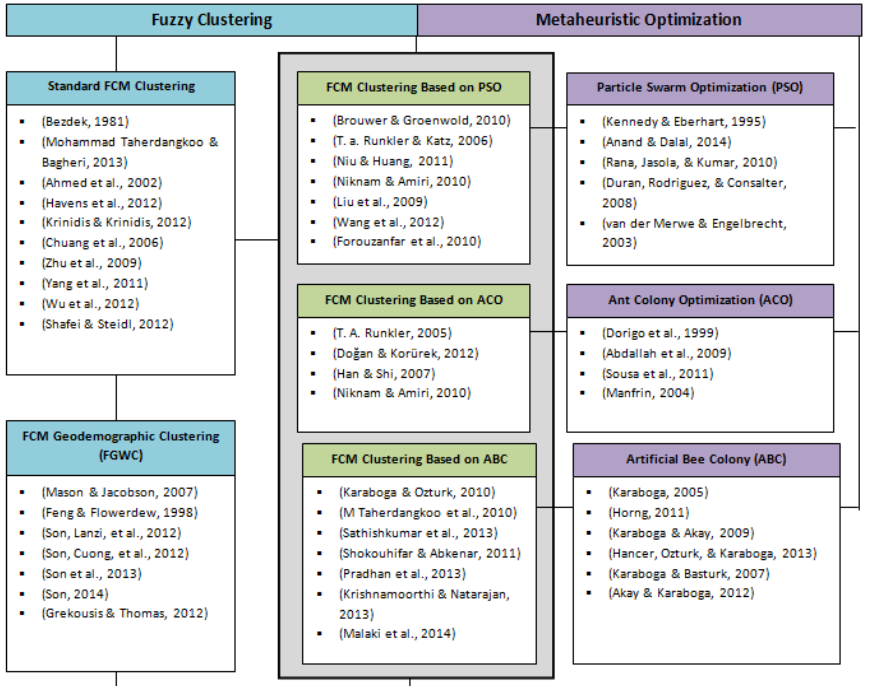
\includegraphics[width=0.49\textwidth]{litmap.png}}
		\caption{Contoh peta literatur (\textit{literature map})}
		\label{lit_map}
	\end{figure}

\section{Mostrar comparaciones}

Mostrar comparaciones, constrastes y diferencias

\section{Muestra datos multivariados}

Cruza las variables. 

\section{No PAY}

No utilices pay nunca. 

\begin{itemize}
	\item Atas = 19mm (0,75")
	\item Bawah = 43mm (1,69")
	\item Kiri = Kanan = 14,32mm (0,56")
\end{itemize}
	
Nunca. 

\section{Realizar gráficos que se expliquen por sí solos}



\subsection{Format Gambar}
	
	Gambar diberi nomor dengan menggunakan angka Arab. Keterangan gambar harus dalam font biasa ukuran 8. Keterangan gambar dalam satu baris diletakkan di tengah (\textit{centered}), sedangkan keterangan multi-baris harus dirata kiri dan kanan. Keterangan gambar dengan nomor gambar harus ditempatkan setelah gambar terkait, seperti yang ditunjukkan pada Gambar \ref{fig_sample}.

	\begin{figure}[htbp]
		\centerline{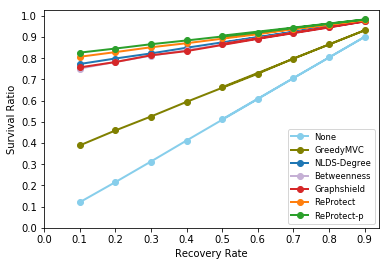
\includegraphics[width=0.45\textwidth]{figure.png}}
		\caption{Contoh keterangan gambar}
		\label{fig_sample}
	\end{figure}



\subsection{Format Tabel}
	
	Tabel diberi nomor menggunakan angka romawi huruf besar. Keterangan tabel di tengah (\textit{centered}) dan dalam font biasa berukuran 8 dengan huruf kapital kecil. Setiap kata dalam keterangan tabel menggunakan huruf kapital, kecuali untuk kata-kata pendek seperti yang tercantum. Keterangan angka tabel ditempatkan sebelum tabel terkait, seperti yang ditunjukkan pada Tabel \ref{tbl_sample}.

	\begin{table}[htbp]
		\caption{Contoh keterangan tabel}
		\begin{center}
		\begin{tabular}{|c|c|c|c|}
			\hline
			\textbf{\textit{Judul kolom}} & \textbf{\textit{Judul kolom}} & \textbf{\textit{Judul kolom}}& \textbf{\textit{Judul kolom}} \\
			\hline
			& Contoh isian tabel$^{\mathrm{a}}$& &  \\[2ex]
			\hline
			\multicolumn{4}{l}{$^{\mathrm{a}}$Contoh catatan kaki pada tabel.}
		\end{tabular}
		\label{tbl_sample}
		\end{center}
	\end{table}




\subsection{Format Persamaan/Rumus}
	Persamaan secara berurutan diikuti dengan penomoran angka dalam tanda kurung dengan margin rata kanan, seperti dalam (1). Untuk Microsoft Word, gunakan \textit{equation editor} untuk membuat persamaan. Untuk membuat persamaan lebih rapat, gunakan tanda garis miring ( / ), fungsi pangkat, atau pangkat yang tepat. Gunakan tanda kurung untuk menghindari kerancuan dalam pemberian angka pecahan. Beri spasi tab dan tulis nomor persamaan dalam tanda kurung seperti tertulis pada Persamaan \ref{equation1} berikut: 

	\begin{equation}	
		Q = \sum^n_{i=1} \frac{x_i - \bar{x}}{y_i - \bar{y}}
		\label{equation1}
	\end{equation}	


\section{Format Referensi/Pustaka}

	Setiap referensi/pustaka diberikan penomoran dan ditulis di dalam kurung siku, misalnya [1]. Semua item referensi berukuran font 8 pt. Silakan gunakan gaya tulisan miring dan biasa untuk membedakan berbagai perbedaan dasar seperti yang ditunjukkan pada bagian Referensi. Menggunakan inisial nama pertama penulis dan nama lengkap mereka yang terakhir. Misalnya "D. Harahap".

	Ketika mengacu pada item referensi, silakan menggunakan nomor referensi saja, misalnya [2]. Jangan menggunakan "Ref. [3]" atau "Referensi [3]", kecuali pada awal kalimat, misalnya "Referensi [3] menunjukkan bahwa ...". Dalam penggunaan beberapa referensi masing-masing nomor diketik dengan kurung terpisah (misalnya [2], [3], [4] - [6]).

	Sebagai catatan, penggunaan langsung referensi yang dicontohkan pada \textit{template} ini dapat dilihat pada Daftar Pustaka. \cite{pustaka1,pustaka2,pustaka3,pustaka4,pustaka5}

\subsection{Buku}

	\textit{Elemen kutipan:}

	Nama penulis pertama atau inisial. Nama atau nama organisasi, Judul buku diikuti oleh fullstop jika tidak ada pernyataan edisi, atau koma jika ada pernyataan edisi, ed., Edisi (kecuali yang pertama). Tempat kota publikasi : penerbit, tahun terbit.

	\textit{Contoh \cite{pustaka1}:}

	A. E. Brouwer and W. H. Haemers, Spectra of Graphs. New York: Springer, 2012.

\subsection{Bagian/Bab dalam Buku}

	\textit{Elemen kutipan:}

	Nama penulis pertama atau inisial. Nama keluarga, "Judul bab," Judul dari buku, ed, Edisi. (Kecuali yang pertama)  jilid, volume jika tersedia, Ed. Editor jika tersedia, Tempat publikasi: Penerbit, Tahun Terbit, pp. Bab atau halaman pertama dan terakhir artikel.

	\textit{Contoh \cite{pustaka2}:}

	P. Shakarian, A. Bhatnagar, A. Aleali, E. Shaabani, and R. Guo, The Independent Cascade and Linear Threshold Models. Cham: Springer International Publishing, 2015, pp. 35–48.

\subsection{Jurnal}

	\textit{Elemen kutipan:}

	Nama penulis pertama atau inisial. Nama Keluarga, "Judul artikel," Judul Jurnal, vol.volume (nomor penerbitan), halaman pertama dan halaman terakhir artikel, tanggal bulan tahun penerbitan jika tersedia.

	\textit{Contoh \cite{pustaka3}:}

	C. Chen, H. Tong, B. A. Prakash, C. E. Tsourakakis, T. Eliassi-Rad, C. Faloutsos, and D. H. Chau, “Node immunization on large graphs: Theory and algorithms,” IEEE Transaction on Knowledge and Data Engineering, vol. 28, no. 1, pp. 113–126, Jan 2016.

\subsection{Seminar/\textit{Proceeding}}

	\textit{Elemen kutipan:}

	Nama penulis pertama atau inisial. Nama keluarga, "Judul paper," dalam seminar Judul, Nama Depan Nama Terakhir Editor jika tersedia, Ed. Tempat Publikasi: Penerbit jika tersedia,  tanggal diterbitkan , halaman pertama dan terakhir paper.

	\textit{Contoh \cite{pustaka4}:}

	A. W. Wijayanto and T. Murata, “Learning adaptive graph protection strategy on dynamic networks via reinforcement learning,” in 2018 IEEE/WIC/ACM International Conference on Web Intelligence (WI), ser. WI 2018. New York, USA: IEEE, Dec 2018, pp. 534–539.

\subsection{Sumber Elektronik (\textit{Website})}

	\textit{Elemen kutipan:}

	Penulis. (tahun, bulan). Judul. [Jenis Perantara]. Available : site/path/file.

	\textit{Contoh \cite{pustaka5}:}

	Facebook. (2017, 3) How does news feed decide which stories to show? [Online]. Available: https://www.facebook.com/ help/166738576721085
	
% Elemen daftar pustaka yang disimpan dalam file Proposal.bib
\bibliographystyle{IEEEtran}
\bibliography{Proposal}

\end{document}
